\chapter{Simulation and Collider Physics}

\section{Introduction}

In the previous chapter, we outlined principle aspects and fundamental assumptions of the  standard model, 
in addition, a considerable amount of physics is still required to reach a practical
 description of what occurs inside of a physics experiment. The goal of this section is
 to connect the matrix elements $\mathcal{M}$ from the quantum field
theoretic description  of the Standard Model to the Monte Carlo simulations used to test our understanding of 
a given theory in the conventions used by experiental high energy physics. First, we will discuss the how
we can compare the matrix amplitudes with the observations in a physical detector. 
After, we will the discuss the considerations that must be made for the fact the
 LHC collides hadrons rather than fundamental particles. We will discuss the
 framework used to describe the particles actually observed in the detector after the
 hard scattering occurs where perturbative physics breaks down and  calculations from first
principles cannot be performed. Generic principles for parton showering and hadronization
 models will be examined. 

\section{From Matrix Elements to Cross Sections} 

In high energy experimental particle physics the key quantity (besides particle quantum numbers and masses) is the
cross section $\sigma$ of the process. This is the rate or in essence, the probability that an event occurs. It is the proportionality between the number of observed collisions and the rate at which the Large Hadron Collider
 delivers collsions $L$ (the luminosity)  expressed simply as:
\begin{align*}
N_{events} = L \times \sigma
\end{align*}
cite-peskin
Consider a target of particles type $A$ and density $\rho_A$ and aim particles type 
$B$ with density $\rho_B$. If the lengths of the bunches of particles are $l_A$ and $l_B$ 
then the cross section of the processes is defined for a beam with cross-sectional area as:
\begin{align*}
\sigma \equiv \frac{N_{events}}{\rho_A l_A \rho_B l_B A}
\end{align*}
Inverting this and assuming that we have constant density along the beams length:
\begin{equation}\label{eq:sigma}
N_{events} = \frac{\sigma N_A N_B}{A} = \sigma{N_A n_B}
\end{equation}
by comparing this with the relation for $N_{events}$ above containing luminosity, we see the
 luminosity is in effect counting the number of colliding particles per unit area.
 More incident particles and a more focused beam means more scattered events. 
In the last equality we have introduced the impact parameter density $n_B$ for
 the incident $B$ particles.

However, the the end results of feynman diagram calculations yield scattering amplitudes
which are matrix elements of scattering a given intial state into a given final state, not
a cross section. We have to further develop the stocastic interaction of two particles into
something more concrete experimentally.
 
First, we need  must think about the quantum fields within the beams that are colliding. To do so we set up two initial 
wave packets $A$ and $B$ in a limit of definite momentum $p_A$ and $p_B$ and evolve them for a very long time 
with the time evolution operator $\exp{(-iHt)}$ and then consider the final state wave packets with the correct final state particles. This in turn will give us the probability amplitude for producing that final state.  
\begin{align*}
\mathcal{P} = |\langle \phi_1 \phi_2 \ldots| \phi_A \phi_B \rangle | ^2 
\end{align*}
Now consider the number of incident particles colliding along the z-axis, but with non-trivial transverse displacement,
also referred to as impact parameters $b_i$. We will take the perspective that $A$ is a target and $B$ is collinear
with the target and account for the shift in position with an explict factor of $\exp(-ib \cdot k_B)$. The properly normalized expression then reads:  
\begin{align*}
|\phi_A \phi_B \rangle = \int \frac{d^3k_A}{\sqrt{2E_A}(2\pi)^3} \int \frac{d^3k_B}{\sqrt{2E_B}(2\pi)^3}\phi_A(k_A)\phi_B(k_B) e^{-ib \cdot k_B} 
\end{align*}
For a single target $A$ and a beam $B$ with with constant impact parameter density $n_B = N_B / A$ we can write the the number of events as
\begin{align*}
N_{events} = \sum_{\text{incident particles } i} \mathcal{P}_i = \int d^2b n_B(b) \mathcal{P}(b) = n_B \int d^2b \mathcal{P}(b) 
\end{align*}
Comparing this to Equation \ref{eq:sigma} we can write the cross section as:
\begin{align*}
\sigma = \int d^2 b \mathcal{P}(b) 
\end{align*}
and the properly normalized differential cross section for scattering into a the infinitesimal final state momentum element is:
\begin{align*}
 d\sigma &= \left( \prod_f \frac{d^3p_f}{(2\pi)^3 2E_f} \right ) \int d^2b \left ( \prod_{i=A,B}
 \int \frac{d^3 k_i }{(2\pi)^3 \sqrt{2E_i}} \phi_i(k_i) \int \frac{d^3 \bar{k}_i}{(2\pi)^3
\sqrt{2\bar{E}_i}} \phi^*_i(\bar{k}_i) \right)\\ 
 &\times e^{ib\cdot (\bar{k}_S - k_B)} | \langle \{ p_f\} | \{k_i \} \rangle |^2 
\end{align*}
We have 6 dummy integrals to do in $\bar{k}$ over the 3 momentums of particle $A$ and $B$
 so count our delta functions. The $d^2b$ integral gives 2 delta functions in the transverse 
momentum $(2\pi)^2 \delta^2(k_B^\perp - \bar{k}_B^\perp)$.  We have 8 delta functions from 
the matrix element enforcing that the process to conserve energy and momentum
 $\delta^4(k_A +k_B - \sum p_f)$\ and in the complex conjugate with the dummy variable
 $\bar{k}$: $\delta^4(\bar{k}_A + \bar{k}_B - \sum p_f)$. Performing the transverse 
integrals in $\bar{k}_B$ sets $\bar{k}_B^T=k_B^T$ which in combination with the transverse
 barred ampltidue delta functions give $\bar{k}_A^T = k_A^T$. The remaining 2 integrals in $z$ require some properties of delta functions:
\begin{align*}
\int d \bar{k}_A^z d \bar{k}_B^z \delta( \bar{k}^z_A + \bar{k}^z_B  - \sum p_f^z) \delta (\bar{E}_A + \bar{E}_B - \sum E_f) 
\end{align*}
We can integrate the first $B$ integral considering $\bar{k}_B^z$ to be a function of
$\bar{k}_A^z$ and writing the barred energy terms in the momentums and masses:
\begin{align*}
\int d\bar{k}_A^z  \delta \left (\sqrt{\bar{k}_A^2 +m_A^2}  + \sqrt{\bar{k}_B^2 + m_B^2} - \sum E_f \right) 
\end{align*}
We now need to use the property that $\delta[f(x)] = \sum_i (\delta(x_i) / |f'(x_i))|$ where $x_i$ are the zeros of the fuction $f(x)$. Note that given our parmeterization from the first delta function $\partial_{\bar{k}_A^z}(\bar{k}_B^2) = - 2 \bar{k}_B^z$.
\begin{align*}
\int d\bar{k}_A^z & \left (\frac{1}{2} \frac{2\bar{k}_A}{\sqrt{\bar{k}_A^2 +m_A^2}}
 - \frac{1}{2} \frac{2\bar{k}_B}{\sqrt{\bar{k}_B^2 +m_B^2}} \right )^{-1}\delta(\bar{E}_A
 + \bar{E}_B - \sum E_f) \\
=& \int d\bar{k}_A^z \frac{1}{\frac{\bar{k}_A}{\bar{E}_A}- \frac{\bar{k}_B}{\bar{E}_B}}
 \delta(\bar{E}_A + \bar{E}_B - \sum E_f) = \frac{1}{\beta_A - \beta_B}
\end{align*}
The 6 remaining integrals in $k_A$ and $k_B$ remain:
\begin{align*}
d\sigma &= \left( \prod_f \frac{d^3p_f}{(2\pi)^3 2E_f} \right ) \frac{|\mathcal{M}|^2}{2E_A2E_B|\beta_A - \beta_B|}
 \int \frac{d^3 k_A }{(2\pi)^3 \sqrt{2E_i}} |\phi_A(k_A)|^2 \\ 
&\times  \int \frac{d^3 k_B }{(2\pi)^3 \sqrt{2E_i}} |\phi_B(k_b)|^2 \delta^4( k_A + k_B - \sum p_f)
\end{align*}
To proceed further, we must consider the quality of measurements made by particle detectors. 
Real detectors cannot measure arbitrarily small spreads in the momentums $k_A+k_B$. 
The measurements made in a realistic experimental setup are not senitive to the
spread of momentum in the initial wave packets $\phi_A$ and $\phi_B$. Given this, we can take the central value $k_A+k_B=p_A+p_B$
to be a good approximation for the delta function. With this approximation, we can move the delta function outside the integral and
perform the integrals using the unit normalization condition of the two fields $\phi_i$:
\begin{equation} \label{eq:dsigma}
d\sigma = \left( \prod_f \frac{d^3p_f}{(2\pi)^3 2E_f} \right ) \frac{|\mathcal{M}|^2}{2E_A2E_B|\beta_A - \beta_B|} (2\pi)^4
\delta^4 \left (p_A+p_B - \sum p_f  \right )
\end{equation}
Let's consider the simple case of $2 \rightarrow 2$ scattering and use the energy delta function 
of the 4 remaining delta functions to compute integral over the final state.
To do so, we go to the center of mass frame where $|p_1| = |p_2|= P$, $\vec p_1 = - \vec p_2$, $E_{cm} = 2P$. We first
integrate $p_2$ to invorce 3-momentum conservation  
\begin{align*}
\int \left( \frac{d^3p_1}{(2\pi)^3 2E_1} \right )\left( \frac{d^3p_2}{(2\pi)^3 2E_2} \right )  (2\pi)^4 \delta^4( P - \sum p_f ) 
\end{align*}
now switching to a spherical integral with a jacobian $p_1^2 dp_1 d\Omega$ where $d\Omega$ is and infinitesimal solid angle.
\begin{align*}
\int \frac{dp_1 p_1^2 d\Omega}{(2\pi)^3 (2\pi)^3 2E_1 2E_2} (2\pi)\delta( E_{cm} -E_1 - E_2)
\end{align*}
here we use the same delta function identity to obtain:
\begin{align*}
\int d\Omega \frac{p_1^2}{(2\pi)^2 2E_1 2E_2} \left ( \frac{p_1}{E_1} + \frac{p_2}{E_2} \right )^{-1} = &\int d\Omega \frac{p_1^2}{(2\pi)^2 2E_1 2E_2} \left ( \frac{E_1E_2}{p_1(E_1+E_2)} \right ) 
\\= &\int d\Omega \frac{p_1}{16\pi^2 E_{cm}}
\end{align*}
Combining the result for the final state integral with Equation \ref{eq:dsigma}:
\begin{align*}
\left (\frac{d\sigma}{d\Omega} \right)_{CM}  = \frac{1}{2E_A2E_B|\beta_A - \beta_B|}  \frac{p_1}{16\pi^2 E_{cm}} |\mathcal{M}|^2
\end{align*}
Now if we assume the masses of the four particles are the same (or negligble at the energies involved) 
and substitute $\beta = p / E$:
\begin{align*}
\left (\frac{d\sigma}{d\Omega}\right)_{CM}  = \frac{|\mathcal{M}|^2}{64\pi^2E_{cm}^2} 
\end{align*}
This is the relation between the rate at which a detector will observe a $2\rightarrow 2$ process proportional to 
the matrix element derived from the feynman diagrams governing the process. 

\section{Luminosity}

%% \begin{equation}
%% L = \frac{f_{rev} n_b N_b^2}{4\pi \sigma_x^* \sigma_y^*} R(\theta_c, \epsilon, \beta^*, \sigma_Z)
%% \end{equation}

\begin{equation}
L = \frac{f}{\pi} \frac{N_p N_{p`}}{n_b} \frac{\gamma}{\sqrt{\beta^*_x \beta^*_y E_x^* E_y^*}}
\end{equation}

\begin{itemize}
\item $f$: revolution frequency of the beams. 
\item $N_p$ the number of protons in the eam
\item $n_b$ the number of proton bunches 
\item $\beta^*_{x,y}$ the trasnverse wavelengthes of the beatatron oscillations
\item $E_{x,y}^*$ the transverse emitance of the beams
\item $\gamma$: relativistic factor
\end{itemize}

To increase luminosity, this parameterization tells us we want a high frequency of collisions, high proton density within
the bunches, small oscillations transverse to the ideal path, and a small average spread in position momentum space. The 
small spread in phase space (low emittance) means the particles are confined to a small area and have roughly the same
 momentum. This result in a high probability of interaction.

\section{Parton Model of Hadron Collisions }

cite:qcd-collider-physics-ellis

For a collision of two protons like that of the LHC (or proton anti-proton for Tevatron) the hard scattering 
process is not between the individual hadrons, but hadron's inner structure: the quarks and gluons. Unlike, 
a lepton collider, where the full four vector is controlled by the collider, the energy of any given hard hadron-hadron
scattering process is probabilistic in nature, as the individual partons have some unknown fraction of the proton energy. 

The cross section for a process for two hadroncs with four-momemntum $P_1$ and $P_2$ can be written:
\begin{equation}
\sigma(P_1, P_2) = \sum_{i,j} \int dx_1 dx_2 f_i(x_1,\mu) f_j(x_2, \mu) \hat{\sigma}_{ij}(p_1, p_2, \alpha_S(\mu), Q)  
\end{equation}
where the momentum of the partons participating in the hard interaction are $p_i=x_i P_i$ $i=1,2$. The scale of the
hard scattering is denoted by $Q$. This would be $m_W$ for $W$ boson production. The $f_i$ are the quark or gluon distributions within the protons. These are the parton distribution function (PDFs). The short distance
cross section $\hat \sigma$ can be calculated as a perturbative series in the asymptotically small running QCD coupling 
$\alpha_S$. The factorization scale $\mu$ is an arbiyrary parameter that is chosen as the boundary between the long
and short distance interaction physics. The boundary at $\mu$ separates the soft emitted partons that should be
considered part of the hadron and the partons emitted at large transverse momentum that should be considered part 
of the hard process. In general, this be set near the order of the process process scaled $Q$. 

If we consider the ratio of the actual $\sqrt{\hat s}$ of the hard process relative to the proton $\sqrt{s}$ we define $\tau$,
the loss of energy between the COM collision of the proton and the individual partons
\begin{align*}
\frac{s}{\hat s}=\frac{(p_1+p_2)^2}{(x_1p_1+x_2p_2)^2} = \frac{2p_1 \cdot p_2}{2x_1x_2 p_1 \cdot p_2} = \frac{1}{x_1x_2} = \frac{1}{\tau}
\end{align*}
Now lets consider the total cross section $\sigma_{TOT}$ which consists of the parton luminosity $L_{ij}$ for two individual
partons $i$ and $j$ and the corresponding cross sections $\sigma_{ij}$. We assume that the cross section $\hat{\sigma}$ is 
only a function of $\hat s$, (a property that holds true for many processes, but not in general). Let $\tau_0$ be the 
minimum $\tau$ at which the process can occur.
\begin{align*}
\sigma_{TOT} &= \sum_{i,j} \sigma_{ij} L_{ij} = \sum_{i,j} \int_{\tau_0}^1  \frac{dL_{ij}}{d\tau}(1)\hat{\sigma}_{ij}  d\tau \\ 
& = \sum_{i,h} \int_{\tau_0}^1 \frac{dL_{ij}}{d\tau} d\tau \left ( \frac{\hat s}{s \tau} \right) \hat{\sigma}_{ij} 
= \sum_{i,j} \int_{\tau_0}^1 \frac{d\tau}{\tau} \left (\frac{1}{s} \frac{dL_{ij}}{d\tau} \right) \left(\hat{s} \hat{\sigma}_{ij}  \right) 
\end{align*}

\begin{figure}
\begin{center}
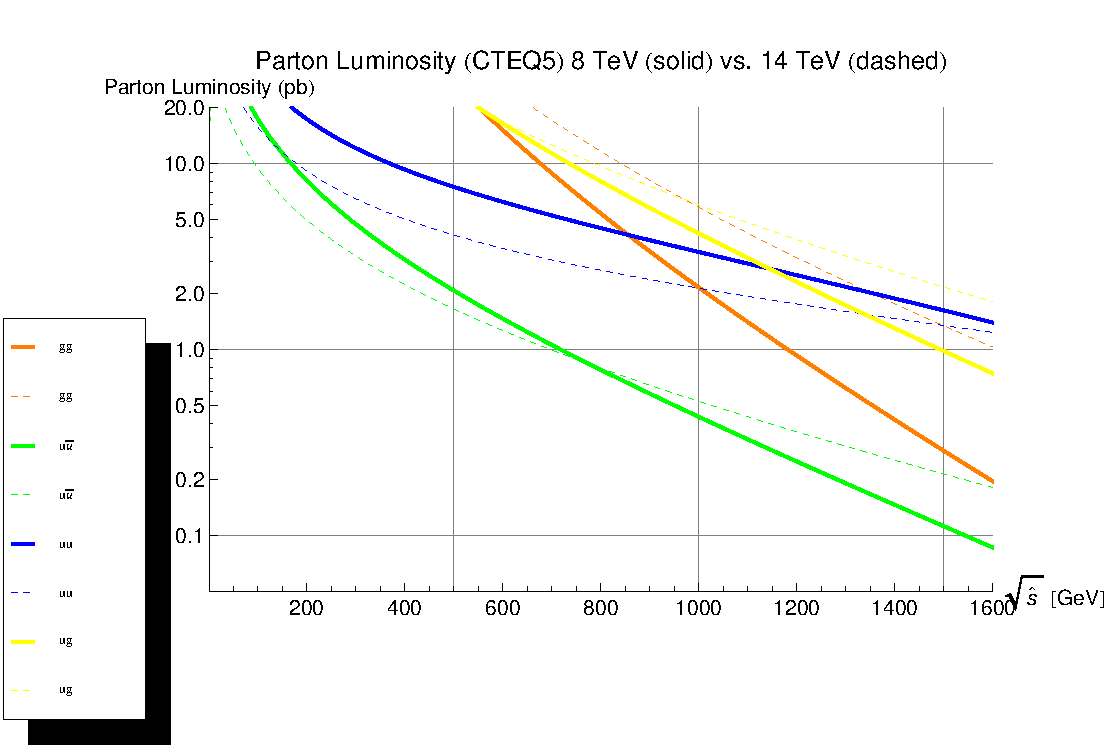
\includegraphics[width=.95\textwidth]{pics/parton_lumi_8TeV_14TeV}
\end{center}
\caption{Contours of the parton luminosity function derived from CTEQ5 parton distribution functions for $\sqrt{s}=8$ TeV and
$\sqrt{s}=14$ TeV. Contours are separated by collions the individual partons in the collision.  }
\label{fig:deltaRcones}
\end{figure}

Here the center term is refered to as the parton luminosity function and contains the parton distribution functions with
some extra accounting for the parton types to avoid double counting:
\begin{align*}
\tau\frac{dL_{ij}}{d\tau} = \frac{1}{1+\delta_{ij}} \int_0^1 dx_1 dx_2 \times \left [ (x_1 f_i(x_1,\mu^2) x_2 f_j(x_2,\mu^2)) + (1 \leftrightarrow 2)) \right ] \delta(\tau - x_1x_2) 
\end{align*}

\section{Kinematic Conventions for Collider Physics} 

In experimental particle physics, due to cylindrical symmetry of our detectors it is preferrable to make a change
from a cartesian energy and momentum parmaterization to  rotationally-symmetric parameteriztion about
the collision access. Furthermore, since the center of mass frame between the two colliding particles is generally moving
relative to the lab frame, we would like parameterization of our problem which is invariant under longitudinal boosts. First, 
we will motivate using hyperbolic functions of rapidity to parameterize energy and momentum. Lets recall define the hyperbolic
trigonometric functions:
\begin{align*}
\cosh(x) &= \frac{e^{x} + e^{-x}}{2} \texttt{ , } \sinh = \frac{e^{x} - e^{-x}}{2} \text{, and }\tanh^{-1}x = \ln \left( \sqrt{\frac{1+x}{1-x}} \right)
\end{align*}
combining cosh and arctanh conveniently gives the relativistic $\gamma$ factor for $x=\beta$:
\begin{align*}
\cosh{(\tanh^{-1}{x})} &= \frac{1}{2} \left ( \sqrt{\frac{1+x}{1-x}} + \sqrt{\frac{1-x}{1+x}} \right ) = \frac{1}{2} \left( \frac{(1+x) + (1 -x)}{\sqrt{1-x^2}} \right)  = \frac{1}{\sqrt{1-x^2}}
\end{align*}
and similarlly dervied:
\begin{align*}
\sinh{(\tanh^{-1}{x})} = \frac{x}{\sqrt{1-x^2}} = x \gamma(x)
\end{align*}
If we define $w = \tanh^{-1}(\beta)$ we can conveniently write the energy and mommentum as:
\begin{align*}
E &= \gamma m = m \cosh{w} \\
|p| &= \gamma m \beta  = m \sinh{w} 
\end{align*}
Now lets re-write a lorrentz boost $\gamma$ along the z-axis in terms of $w$:
\begin{align*} \label{eq:boost}
E' = \gamma (E - \beta p_z)   = E \cosh w - p_z \sinh w \\
p_z' = \gamma (p_z - \beta E) = p_z \cosh - E \sinh w
\end{align*}
We now set $w = y = \tanh^{-1}(\beta_z^*)$ where $\beta_z^*$ is the boost required to reach the frame where the particle is
moving only transversely to the beamline $p_\mu^*$. We can then reach the lab frame by performing
 the transformation from the $*$ frame. First lets write the four vector in the $*$ frame
\begin{align*}
 p_\mu^* &= ( E , p_x, p_y, 0 ) = (\sqrt{p_T^2 + m^2}, p_T\sin \phi, p_T \cos \phi, 0)\\
\rightarrow  p_\mu^{lab} &= (m_T \cosh y, p_T \sin \phi, p_T \cos \phi, m_T \sinh y)
\end{align*}
where $m_T = \sqrt{m^2 + p_T^2}$, $p_T = \sqrt{ p_x^2 + p_y^2}$, and $y$ is the definition of rapidity generally used in particle
physics. In the limit of light masses relative to the  transverse energy of a collision, as is generally
 the case for collisions at the Large Hadron Collider:
\begin{align*}
p^\mu = p_T(\cosh \eta , \sin \phi, \cos \phi, \sinh \eta)
\end{align*}
From the experimental perspective, what is most important about this definition is that there is a simple geometric relation
between pseudorapditiy and the angle of the particle relative to the beam line. To see this, we go back to the definition
of rapidity and take $\beta\rightarrow 1$ or equivalently $|p|=E$:
\begin{align*}
y = \tanh^{-1} ( \beta_z^* ) = \ln \left ( \sqrt{\frac{1+\beta_z^*}{1-\beta_z^*}  }\right ) \approx^{\beta\rightarrow\infty} \ln \left ( \sqrt{\frac{1+p_z/|p|}{1-p_z/|p|}  }\right )
\end{align*}
Now if we consider the angle with the beamline in the lab frame $\theta$ we use a half angle trigonometric identity.
\begin{align*}
1+ \cos \theta = 1 +\frac{p_z}{|p|} = 2 \cos^2 (\theta / 2) \\ 
1- \cos \theta = 1 -\frac{p_z}{|p|} = 2 \sin^2 (\theta / 2)
\end{align*}
combining this with the approximation with massless limit of $y$ we obtain pseudorapidity $\eta$:
\begin{align*}
\eta = \ln \left ( \sqrt{\frac{\cos^2{(\theta/2})}{\sin^{2}{(\theta/2)} }}  \right) = - \ln \left ( \tan \frac{\theta}{2} \right )
\end{align*}
\begin{figure}
\begin{center}
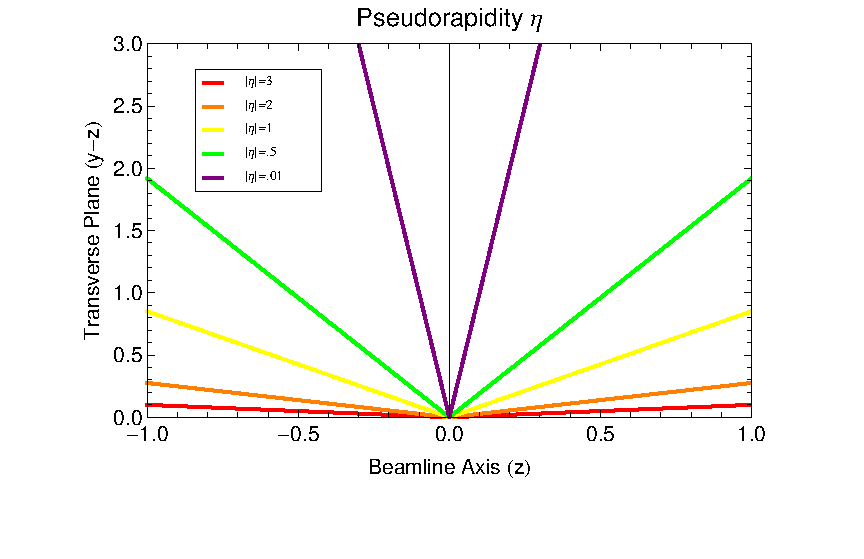
\includegraphics[width=.6\textwidth]{figures/exp_proj/pseudorapidity}
\end{center}
\caption{Lines of constant pseudorapidity in the z-y plane}
\label{fig:pseudorapidity}
\end{figure}
The energies of particles at the LHC are typically negligible in  mass relative to their energies and the approximation $\eta \approx y$ is accurate. This
 has a number of useful applications. Firstly, differences in rapidity are invariant 
under longitudinal lorrentz boosts along the beam axis which can be seen by applying the transformation
 in terms of $\gamma$ factors to $y_1 - y_2$. Given this relation, pseudorapidity provides an
 intuitive geometric interpretation as the angle from the beam axis. The ray extending directly
 transverse from the collision point is $\eta=0$ with symmetric values $\pm|\eta|$ to either
 side of this ray along the z-axis Figure \ref{fig:pseudorapidity}. 
\begin{align*}
\Delta R = \sqrt{ (\Delta \phi)^2 + (\Delta \eta)^2}
\end{align*}
Fixed values of $\Delta R$ form a solid angle ``cone'' extending from the interaction point outward. This can be seen by
 using our definition of $\eta$ to convert from cylindrical coordinates to $(x,y,z)$ and consider the distance relative to the point $(\eta_0,\phi_0)$
\begin{align*}
\Delta R = \sqrt{ \left( \phi_0 - \tan^{-1} (y/x) \right )^2 + \left ( \eta_0 + \log \left( \tan \frac{\cos^{-1} (z/\sqrt{x^2+y^2})}{2} \right) \right)^2 }
\end{align*}

\begin{figure}
\begin{center}
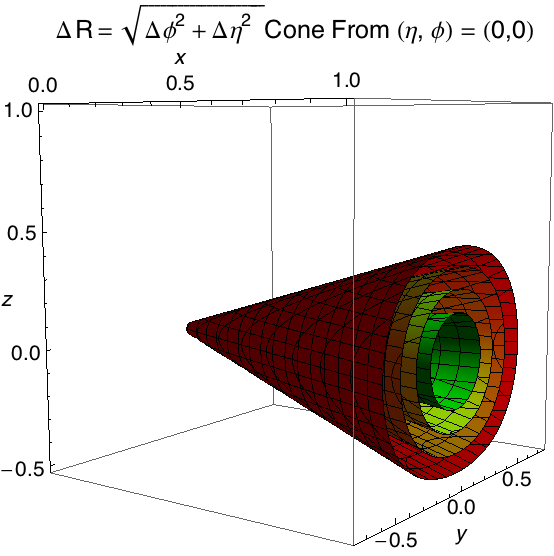
\includegraphics[width=.3\textwidth]{figures/exp_proj/deltaR_cone}
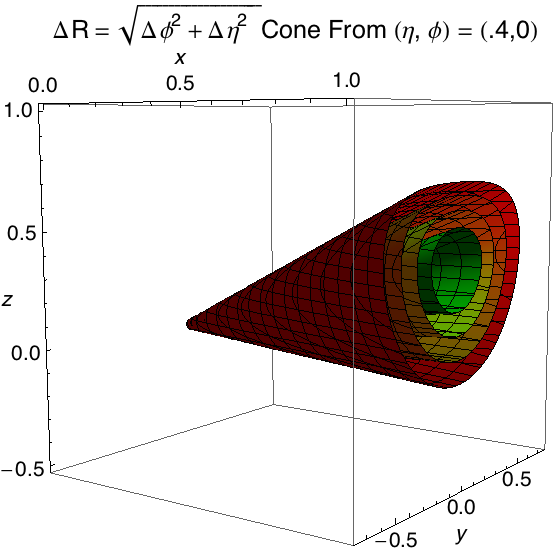
\includegraphics[width=.3\textwidth]{figures/exp_proj/deltaR_cone_eta0p4}
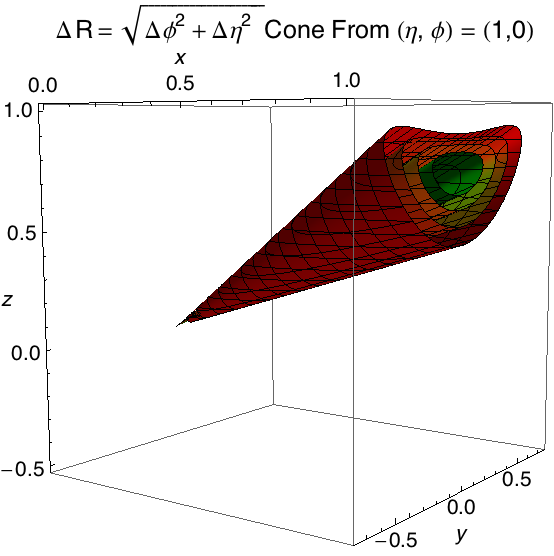
\includegraphics[width=.3\textwidth]{figures/exp_proj/deltaR_cone_eta1p0}
\end{center}
\caption{Contours of constant $\Delta R$ from the $\eta_),\phi_0 = 0,0$}
\label{fig:deltaRcones}
\end{figure}

\section{Showering}

\begin{figure}
\begin{center}
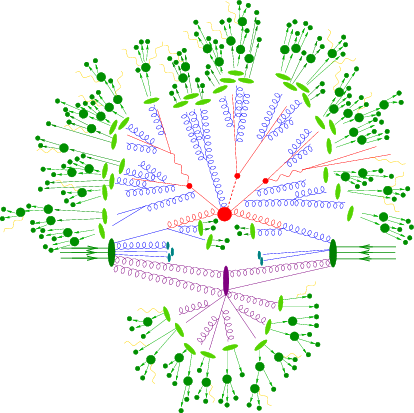
\includegraphics[width=.45\textwidth]{pics/hadronization}
\end{center}
\caption{A graphic depiction of the showering and hadronization process. The incoming protons can be see as the two sets of three
incoming arrows represting the proton quark content.}
\label{fig:showering}
\end{figure}


After the intial hard process is simulated, even if performed at high orders in perturbation theory, we have not described the large multiplicity and variety of particles which result from the showering of free quarks (Fig.~\ref{fig:showering}). We 
might even take for granted (as experimentalistics that is) that high energy proton 
collisions yield collimated showers of hadrons we more commonly refer to as \textit{jets}. 

As the collisions are made between hadrons, the dominant fraction
of the total cross section is governed by the dynamics of QCD. The strength of QCD is set by the strong coupling $\alpha_S(q^2)$ where the $q^2$ dependence arises from loop corrections to the tree level feynman diagram vertices (cite-tully). 
\begin{equation} \label{eq:running_qcd}
\alpha_s(q^2) = \frac{12\pi}{(33-2n_f)\ln{(q^2 /\Lambda_{QCD}^2})}
\end{equation}
Here $n_f$ is the number of flavors of participating fermions in the interaction and $\Lambda_{QCD}=0.1-0.3$. Here we notice two important features. As $q^2$ becomes large, the interaction because asymptotically weak and the physics is perturbative. As $q^2\rightarrow \Lambda_{QCD}$ the theory is
strongly coupled ($\alpha > 1$) and a perturbative approach leaves higher order terms that cannot be neglected 
(cite-ellis-qcd). 

We need a method to evolve the high energy states to some low energy cut off where the physics is clearly non-preturbative. 
This scale is typically taken to be on the order of momentum transfer $t^2 = 1$ GeV$^2$.
This consistutes a natural division of labor for generating physics events between the perturbabtive hard scattering, the approximately perturbative showering, and the non-preturbative physics of hadronization. The terms fragmentation and hadronization are often used interchageably to describe the non-preturbative of this divison. However, in certain contexts, hadronization can refer to the both the parton showering as well as hadron formation. 

In experimental high energy particle physics the term Monte Carlo (MC) is used as a short hand for simulated 
physics samples, however the Monte Carlo method of generating
these samples means something specific. Monte Carlo methods generally rely on using random numbers to simulate 

%% A Monte Carlo algorithm sacrifices the accuracy of the result for a time complexity speed up.
%% This is to be contrasted with a Las Vegas algorithm, which always returns correct results, but the run time is probalistic (and 
%% finite). 
 
(cite-ellis-qcd) The monte carlo method of generating parton branching is stated as: given some 
virtual mass scale $t_1$ and momentum fraction $x_1$ generate
 $(t_2, x_2)$ after one step in the branching evolution. To perform this step-wise evolution of the parton 
branching we need shower evolution equations.

(cite-mrenna-showering) Consider the branching of a particle $a$:  $a\rightarrow bc$ with a 
momentum scale $Q^2$. We denote energy and momentum fraction imparted to particle $b$ as $z$
 such that particle $c$ receives $1-z$. We introduce the momentum
transfer variable reminiscent of (Equation \ref{eq:running_qcd}) $t = \ln (Q^2 / \Lambda^2)$ yielding 
a differential element $dt = d\ln (Q^2) = dQ^2/Q^2$. The
differential probability for the particle $a$ to branch is given:
\begin{align*}
d\mathcal{P} = \sum_{b,c} \frac{\alpha_{abc}}{2\pi} P_{a \rightarrow bc}(z) dt dz 
\end{align*}
where the sum is over all possible branchings and $\alpha$ is the appropriate 
coupling $(\alpha_{EM},\alpha_{S})$  for the branching evaluated at the appropriate scale. We enumerate the kernels that map the momentum fraction from splitting
 to the possible states after branching:
\begin{align*}
P_{q\rightarrow qg} (z) &= C_F\frac{1+z^2}{1-z}   &P_{q\rightarrow q\gamma} (z) &= e_q^2\frac{1+z^2}{1-z}\\
P_{g\rightarrow gg} (z) &= N_C\frac{(1-z(1-z))^2}{z(1-z)} &P_{l\rightarrow l\gamma} (z) &= e_l^2\frac{1+z^2}{1-z} \\ 
P_{g\rightarrow q\bar{q}} (z) &= T_R (z^2 + (1-z)^2)\\
\end{align*}
where $C_F=4/3$ is a color factor, $N_C$ is the number of colors in QCD, $T_R = n_f / 2$ is half the number 
of allowed $q\bar{q}$ flavors. $e_i^2$ is the charge squared of the quark or lepton. 

Lets define an integral over the probability distribution for some fixed $t$ between the
minimally allowable momentum fraction $z_{-}$ and the maximum $z_{+}$ as:
\begin{align*}
\mathcal{I}_{a \rightarrow bc} (t) = \int_{z_{-}(t)}^{z_{+}(t)} dz \frac{\alpha_{abc}}{2\pi} P_{a\rightarrow bc} (z) 
\end{align*}
From this here we can find the total probability of branching as a sum over the
possible branching states $p_{branch} = \sum_{bc} \mathcal{I}_{bc}(t)$. If we consider the probabiity of no branching occuring $(1-p_{branch})$ in some finite
interval $(t,t_0)$ as the product of differential time steps $\delta t$, we obtain an exponential:
\begin{align*}
\mathcal{P}_{no-branch}(t_0,t) = \prod_{\delta t \in (t,t_0)} (1-p_{\text{branch}}) &\approx \lim_{N\rightarrow \infty} 
\sum_{k=0}^{N} \frac{N!}{(N-k)!k!} 1^{N-k}(-p_{\text{branch}})^k  \\
&= \sum_{k=0}^{\infty} \frac{1}{k!} (-p_{branch})^k = \exp{(-p_{branch})}
\end{align*}
Such that the total probability of not branching within a givern $t$ interval is given:
\begin{align*}
\mathcal{P}_{no-branch}(t_0,t) = 
\exp { \left ( - \int_{t_0}^{t} dt' \sum_{b,c} \mathcal{I}_{a\rightarrow bc} (t')   \right )} = S_{a}(t)
\end{align*}
Where we have introduced the notation $S_a(t)$ for what is referred to as the Sudoakov form 
factor (cite-sudakov). With this single parameterization we can write the probability of not branching as a ratio of $S_a(t)$ functions (since the ratio of exponentials will just alter the integral bounds):
\begin{align*}
\mathcal{P}(t_2, t_1) = \frac{S_a(t_{2})}{S_a(t_1)}
\end{align*}
Note here that $t$ is not time, but rather serves a proxy for time, where the
final state showering occurs from an intial $t_{max}$ set by the hard scattering and progressively becomes smaller through the branching process.   

The Monte Carlo process generates a random number $\mathcal{P}$ and solves for $t_2$ in terms
of $t_1$. The process is then applied to the newly branched particles $b$ and $c$. If $t_2$ is smaller than the scale
 set for hadronization, then the showering process terminates. Eventually from the monotonicity of $t_i$ the cascade
terminates and the generation process is handed off to hadronization.

\section{Hadronization} 

When the quark model, the eight-fold way, was orignally introduced in 1961, it was a large simplification of the space of observed  particles. Each combination of possible light quarks was observed in nature (the third generation had not 
yet been discovered). However, a  single ``bare'' quark had never been observed despite experimental efforts. Today
we understand that it is the inherent nature of the strong force that prevents light quarks from being liberated from their 
hadronic bound states. As an interesting side note, the discovery of the top quark, who's width is  larger than $\Lambda_{QCD}$, 
will decay before hadronization takes place allowing for the study of a ``bare'' quark. In this section, we breifly discuss
 the way  monte carlo simulation models the non-preturbative confinement of quarks.

(cite-ellis) When we leave the showering process, we are left with a large number of virtual particles on the order of the cutoff $t_{min}$. Although this
parameter is unrelated to the hadronization process, an ideal hadronization model would use the chosen value of $t_{min}$ to compensate for
 effects of having a hard cutoff value for the showering. 
 As $t_{min}$ is increased, there are fewer particles that are increasingly off-shell. These virtual particles should be
 able to hadronize, however, the favored values of $t_{min}$ to begin the hadronization step tend to be a few times the
 scale of hadronization $\Lambda_{QCD} \approx 0.1 - 0.3$ GeV. This is suggestive that the extensions of perturbation theory
 are more reliable than models of hadronization.

(cite-mc-review) It is important to state that there are only models of hadronization and no calculations from first principles. 
Even lattice QCD calculations which are made on euclidean space times fail for processes which are inherently minkowskian 
such as hadron formation. Two main categories of hadronization models exist. The string 
model which transforms virtual particles directly into hadrons and the cluster model which uses in intermediate clustering step before
the conversion to hadrons. 

\begin{figure}
\begin{center}
\includegraphics[width=.9\textwidth]{pics/linear_confinement}
\end{center}
\caption{The static quark anti-quark potential as measured from lattice qcd calculations. An additional $f/R^2$ term is included to
account for known artifacts from performing the measurement on a lattice. However, the linear at large $R$ (in units
of fm  is clearly visible. (left) the quark anti-quark potential 
including the coloumb term at short distances (right)}
\label{fig:linear_confinement}
\end{figure}

\begin{figure}
\begin{center}
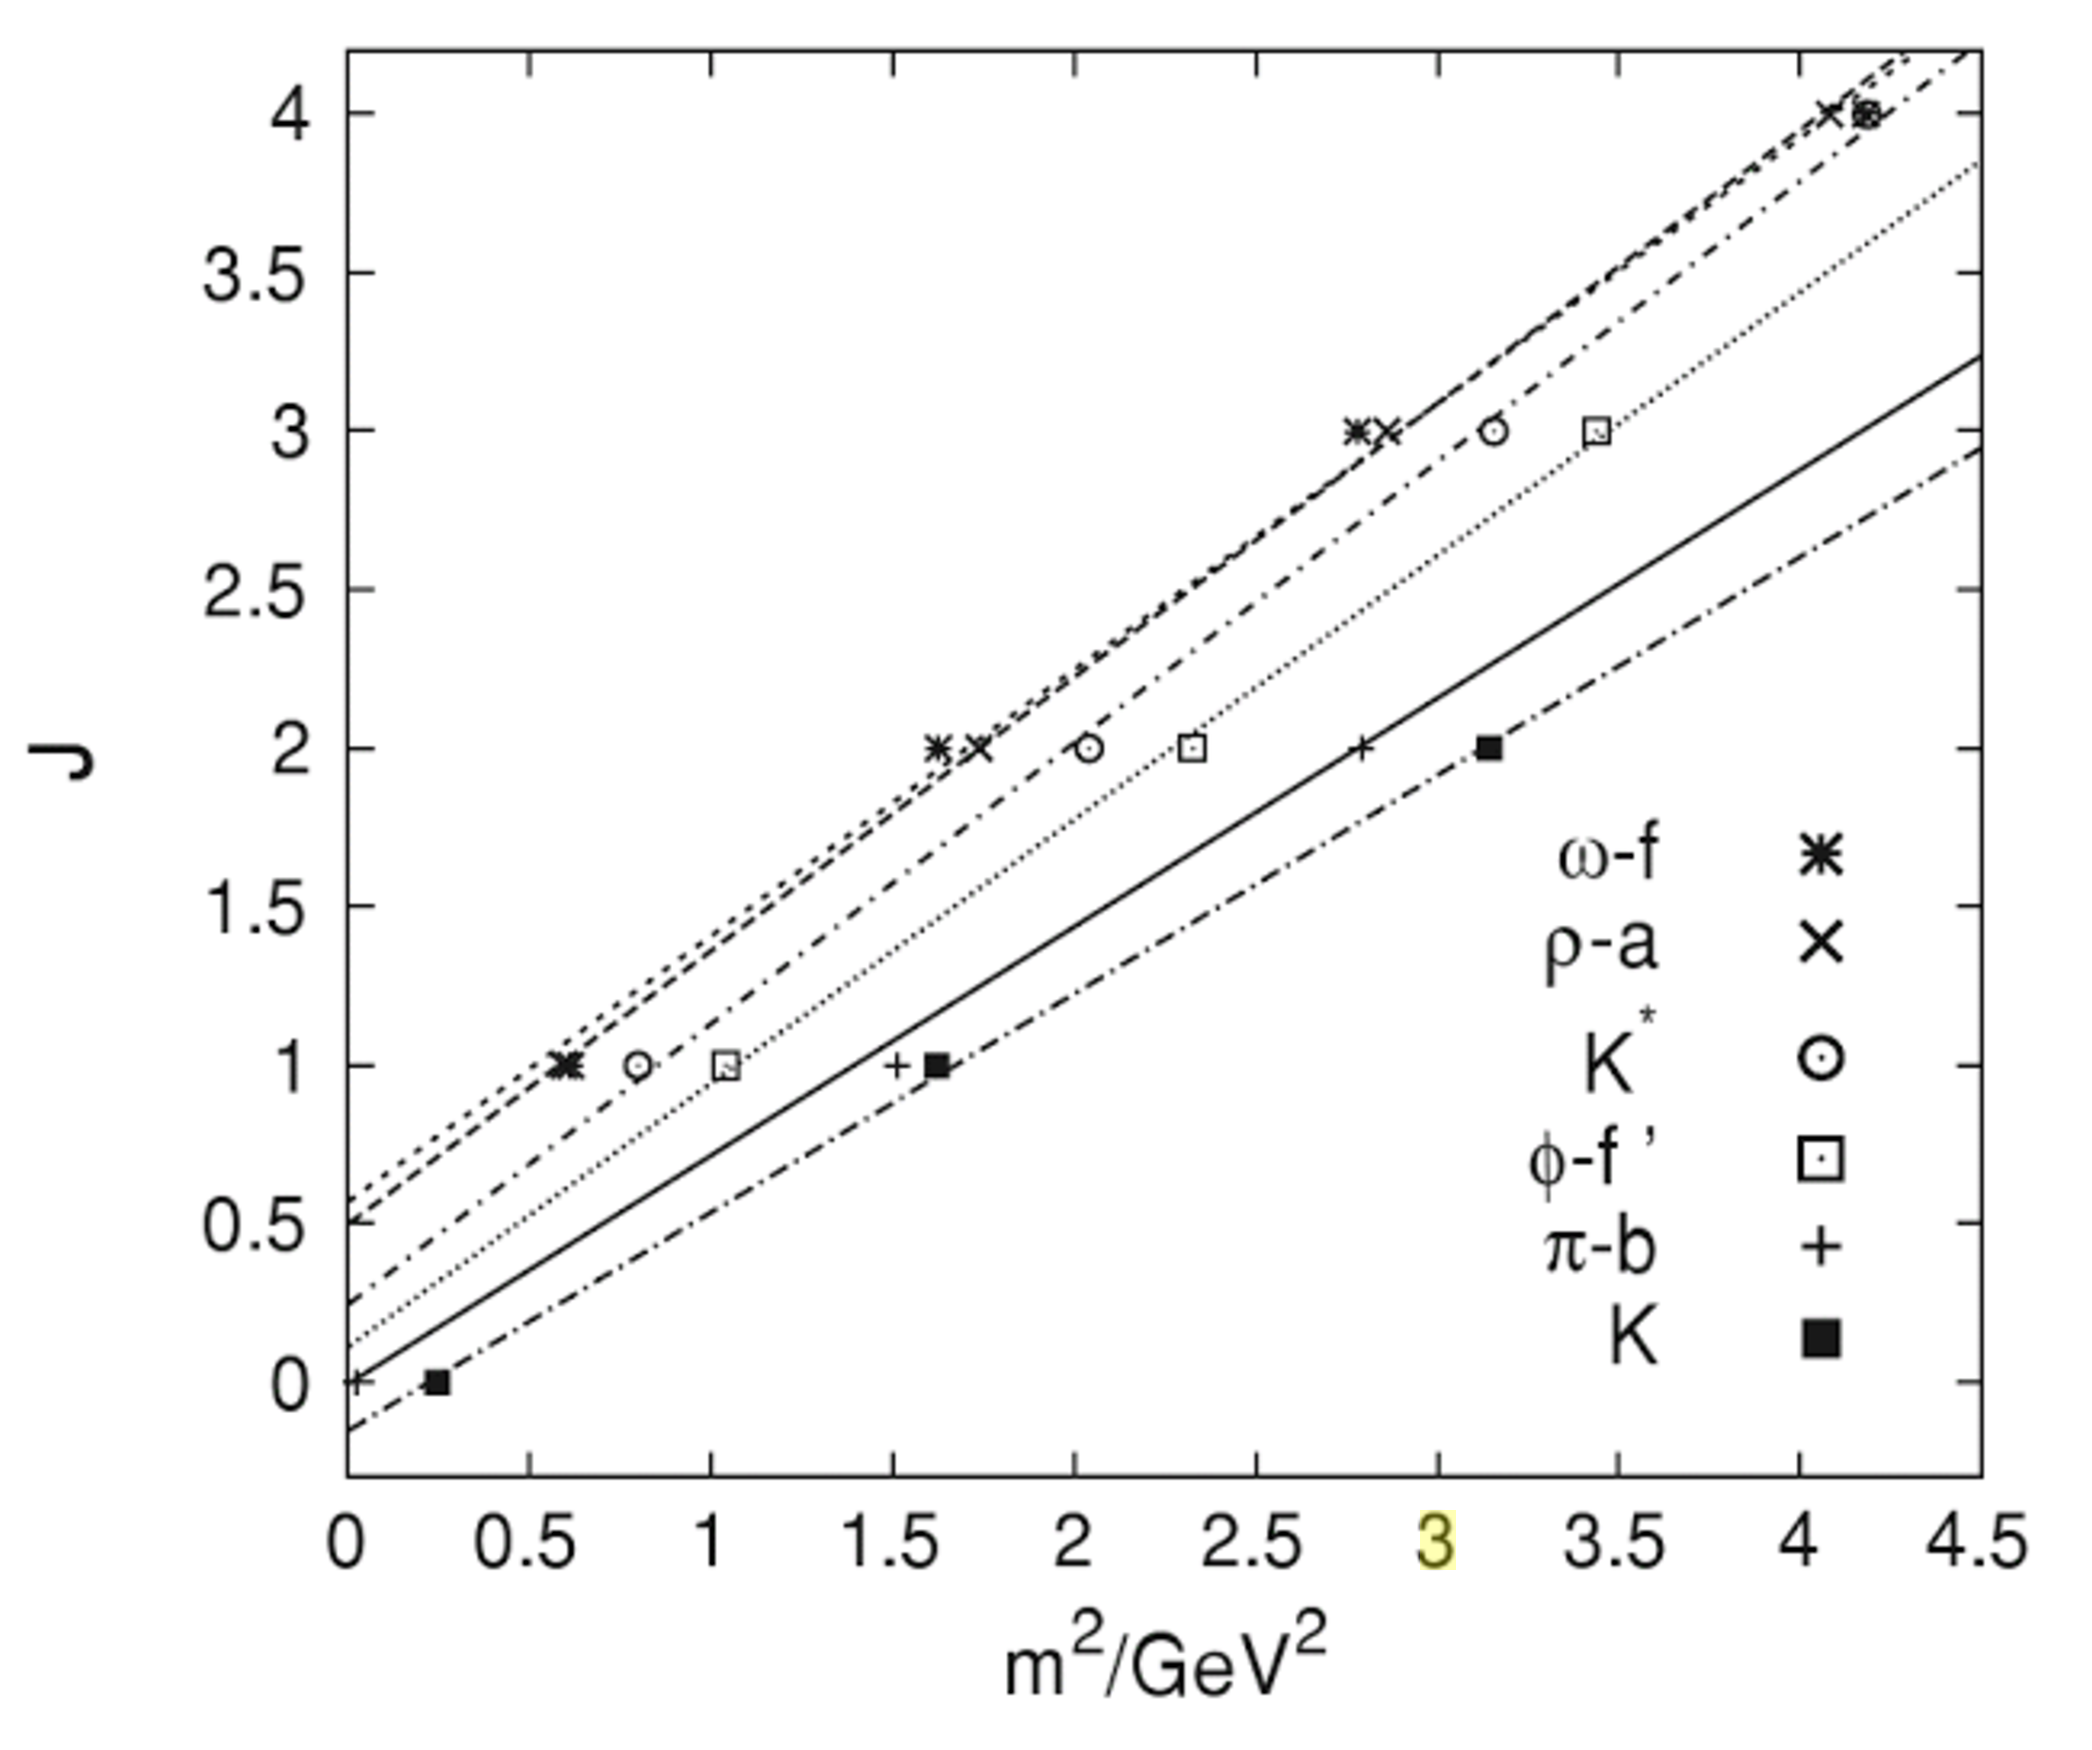
\includegraphics[width=.55\textwidth]{pics/regge_trajectories}
\end{center}
\caption{When the spin  of mesons are plotted against their mass squared a linear relationship is found with nearly the same scaling. These lines are
known as Regge trajectories.  }
\label{fig:regge}
\end{figure}

The string model, the most well known of which is the Lund String Model (cite-lund-string), relies on an assumption of linear confinement. One expects
a linear potential $V(r) = \kappa r$ at long distances, where the string constant $\kappa \approx 1$~ GeV/fm $\approx .2$ GeV$^2$. In general, 
there is an additional coulomb potential at shorter distances (Figure \ref{fig:linear_confinement}). The Lund model assumes that this term is negligible
in hadron formation. 

One motivation for the linear confinement comes from the linear relationship between the spin of mesons $J$ and their $m^2$ (Figure \ref{fig:regge}). To explain why,
lets consider a spinning rod of mass constant density $\sigma$ (that is to say linearlly scaling energy with length) and length 2$R$, we have can calculate the
total energy as:
\begin{align*}
m = E &= 2 \int_0^R \gamma(r) \sigma dr = 2 \int_0^R \frac{\sigma dr}{\sqrt{1 - \frac{r^2}{R^2}}} = \pi \sigma R 
\end{align*}
and if we calculate the angular momentum
\begin{align*}
J = 2 \int_0^R r \beta \gamma (r)\sigma dr  =  2 \int_0^R \frac{\sigma r \beta }{\sqrt{1- \beta^2(r)}} =  \frac{2}{R} \int_0^R \frac{\sigma r^2 }{\sqrt{1- \frac{r^2}{R^2}}} = \frac{1}{2} \pi \sigma R^2 
\end{align*}
by comparison we see that $J=\frac{1}{2\pi\sigma}m^2 = \alpha m^2$. From data this constant relationship is found to be $\alpha = 0.9$ GeV/fm. This relationship
was also found to be accurate in static calculations of the quark anti-quark potential in lattice QCD as shown in  Figure \ref{fig:linear_confinement}. 
\begin{figure}
\begin{center}
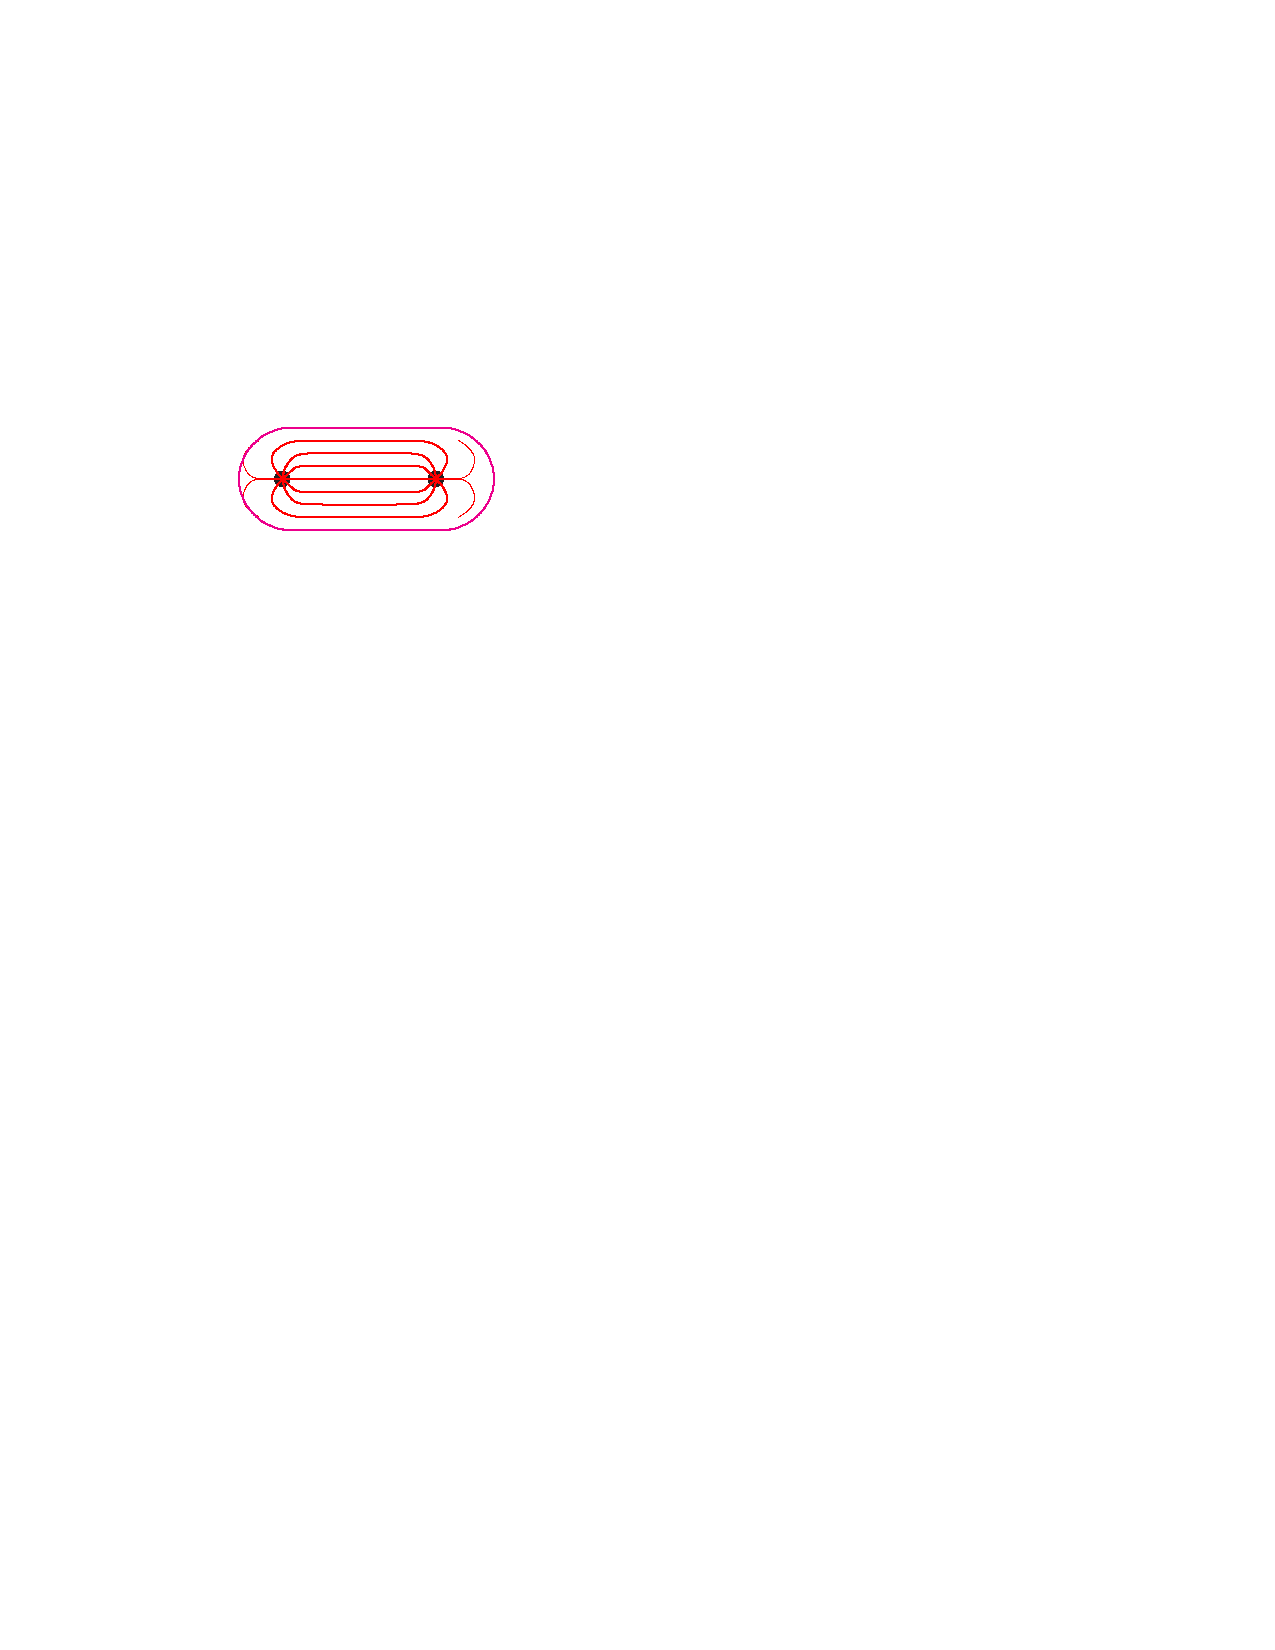
\includegraphics[width=.45\textwidth]{pics/flux_tube}
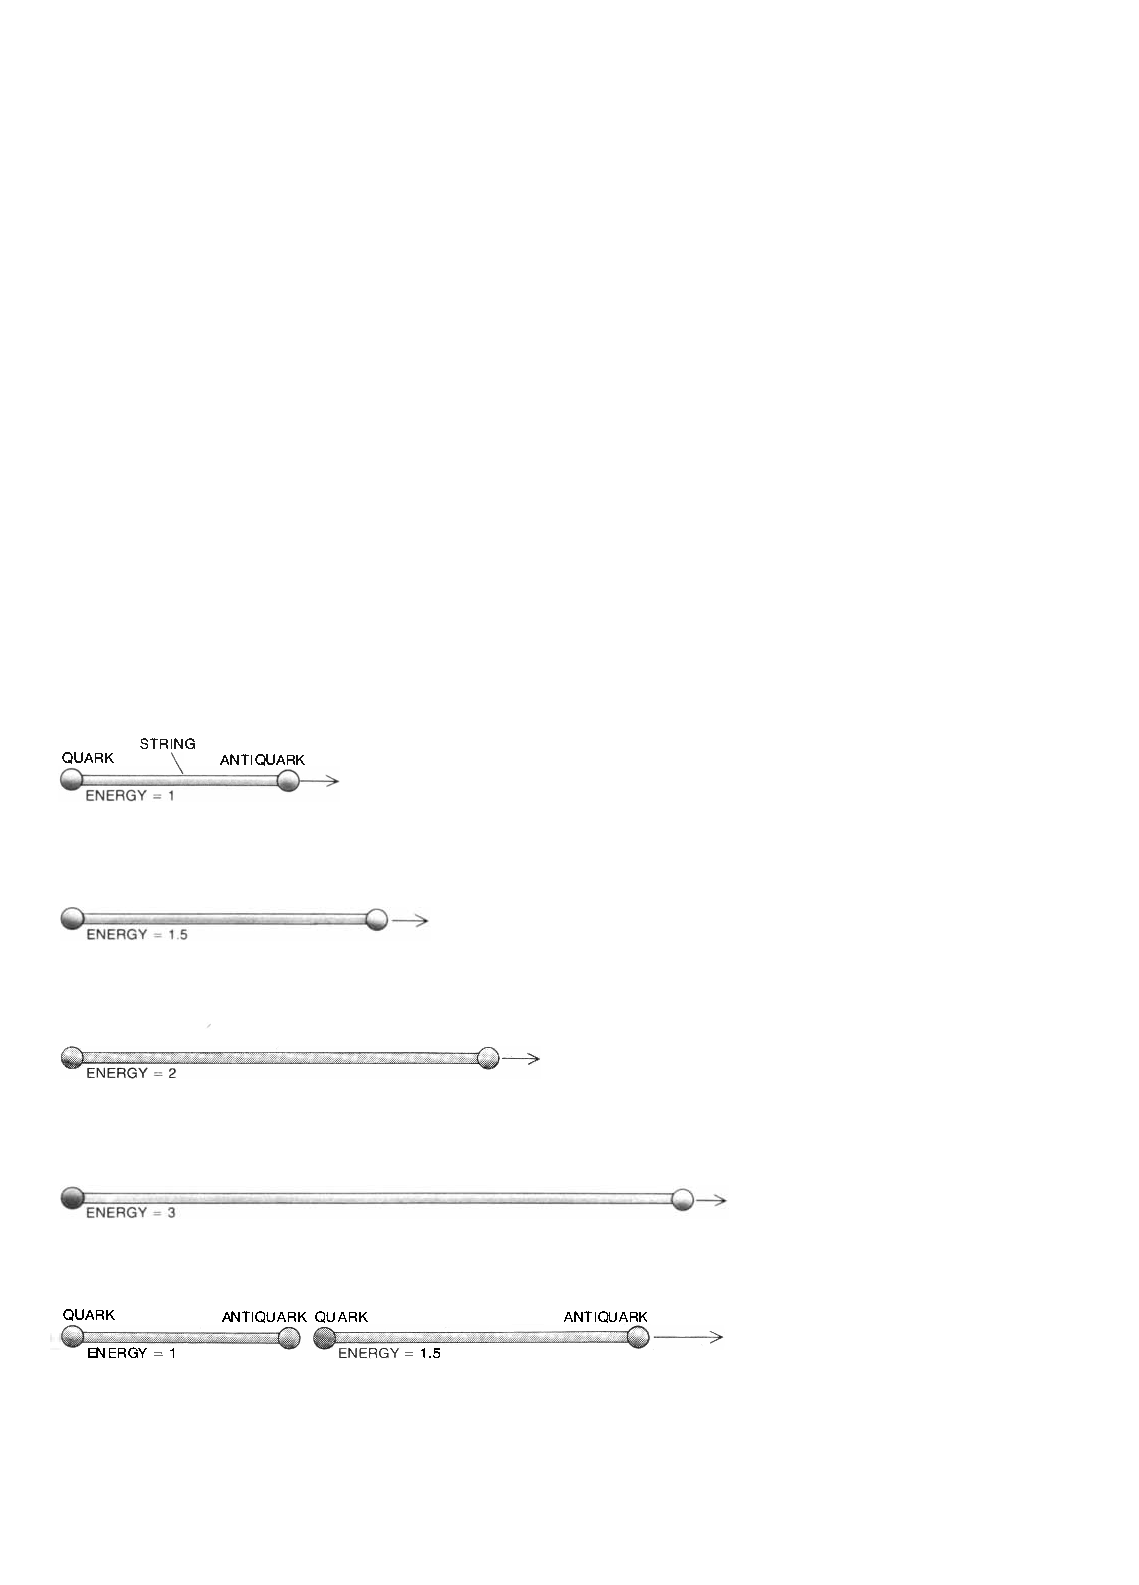
\includegraphics[width=.45\textwidth]{pics/string_stretch}
\end{center}
\caption{The flux between a quark and anti-quark (left) A simple model of quarks as the ends of a string. As an 
attempt is made to separate the two quarks, the string breaks producing two new ends i.e. quarks (right) (cite-string-sretch) }
\label{fig:flux_tube}
\end{figure}
It is important to note that string model of hadronization should not be confused with the strings of string theory where strings serve as the fundamental .  The linear
 confinement of QCD is best visuallized as a color flux tube being stretched between a quark and anti-quark (Figure. \ref{fig:flux_tube}). These flux lines are similar
to those of the equipotential lines between a positive and negative electric charge but with a charactersitic $~r$ dependence rather than $~1/r$. 
As the two quarks are increasingly separated in space, the flux tube is stretched maintaining constant energy per unit length $\kappa$. The lorrentz covariant and
causal description of this energy flow uses a massless one dimensional string that parameterizes the axis of a cylindrically symmetric flux tube. 
\begin{figure}
\begin{center}
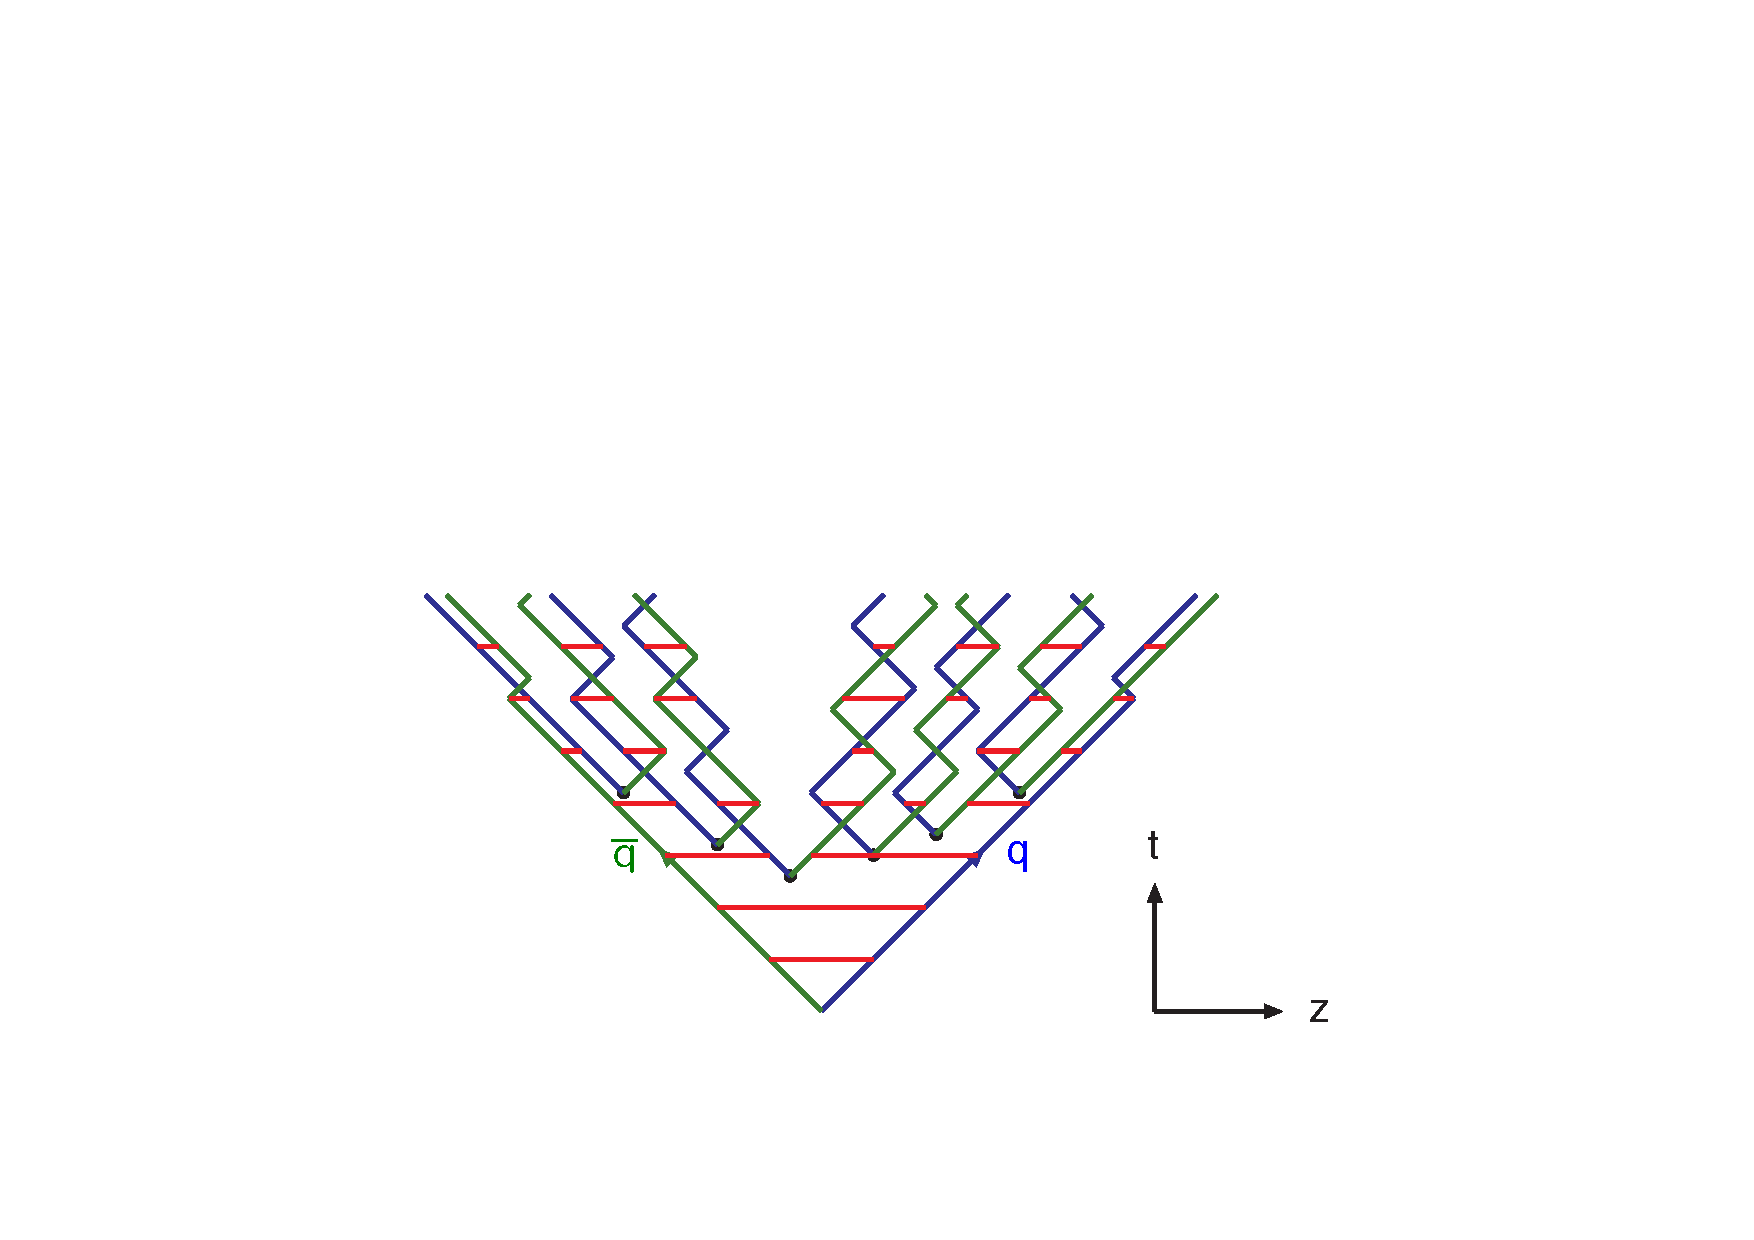
\includegraphics[width=.65\textwidth]{pics/lund_model}
\end{center}
\caption{The 1+1 dimensional propogation of the hadronization process beginning form a quark anti-quark pair.  }
\label{fig:lund}
\end{figure}
In the simple case of quark anti-quark production in the (Figure \ref{fig:lund}), the two quarks separate 
from each other along the $z$ axis and the potential energy stored in the 
string increases. When the potential energy is large enough, the string can break through the production
 of a new quark anti-quark pair. These breaks typically occur between 1 and 5 fm in the rest
 frame of the pair, however in the lab frame these processes are highly length contracted. 
After the break, widening regions of no flux arise. By the end of the process, the string has been broken into many
segements through the creation of $q\bar{q}$ pairs. Hadrons are formed by a quark from one break and the anti-quark
of an adjacent break. The energy-momentum picture is derived from the space-time picture through the string
tension as: (cite-mc-review)
\begin{align*}
\left |\frac{dE}{dz}\right|  = \left|\frac{dp_z}{dz}\right| = 
\left|\frac{dE}{dt}\right| = \left|\frac{dp_z}{dt}\right|  = \kappa
\end{align*}
This is to say that the hadron has energy equal to the string constant times the separation in space between the 
two quarks and momentum equalt o the string cosntant times the separation in time. Based on this relation we enforcing
 the hadrons to be formed on shell requires the constuant two breaks that build a hadron to be causally separated i.e. space-like. 
\begin{align*}
m_T^2 = E^2 - p_z^2 = \kappa((\Delta t)^2 - (\Delta z)^2) > 0 
\end{align*}
This also means that as the hadron propagates, the kinks in the hadron pair will always occur with the same separation
(the bound rectanges in Figure \ref{fig:lund} will always have the same area). This corresponds the hadron remaining on shell.

The string model contains a large number of parameters related to flavor properties and must determined from data

The cluster model is based on the precontainment properties of parton showers which lead to  color singlet clusters. The cluster hadronization begins with
non-preturbative splitting of gluons into quark anti-quarks pairs. Clusters are formed from color-connected pairs. Most clusters under go two body phase-space decays, 
with heavier clusters decaying first to lighter clusters. Cluster models tend to describe the data less accurately than 
string models, but using fewer parameters.

The incredibly dense and active enviroment of hadronic collisions could lead to significant collective effects
 which are not considered in current hadronization models.
\section{Hadron Decay} 

(cite-mc-review) Once we the final hadron picture, the hadrons must be decayed into particles which are stable on the length scales of the detector. That is,
the final particles that measured by the individual sub-detectors.  It might seem simple that the generators could use
 known branching ratios from the extensive Particle Data Group tables on particle decays (cite-pdg-tables), however, 
this information is often incomplete. The least documented decay modes are excited multiplets including heavy quarks (bottom and charm).

One important choice that must be made for different generators is which hadrons to include in their simulation. For starters,
all simulators include the lighetsts pseudoscalar, vector, scalar, event and odd charge conjugation pseudovector and tensor multiplets of light mesons. These decisions 
must be made carefully as in certain models the exclusion of any members of a given multiplet cause unphysical rates of isospin violation. 

\section{Jet Clustering}

\begin{figure}
\begin{center}
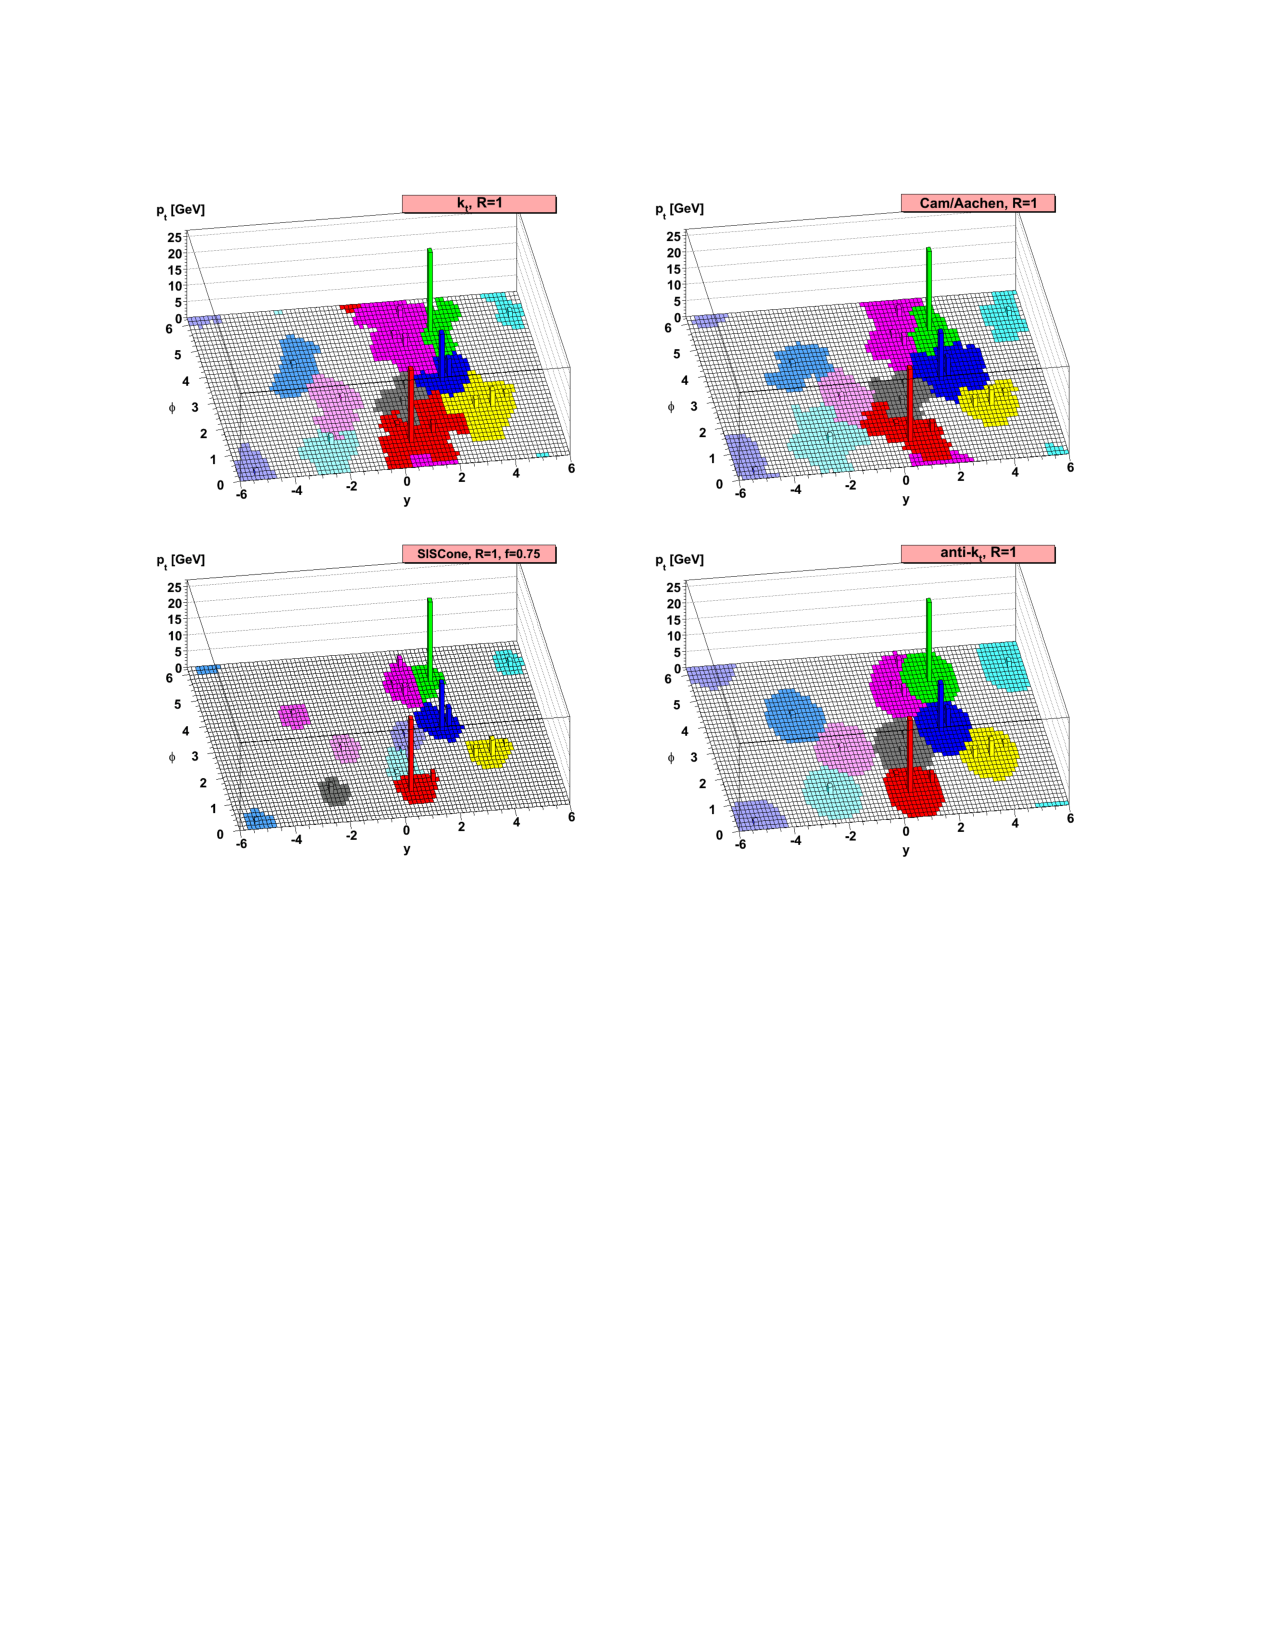
\includegraphics[width=.75\textwidth]{pics/antikt}
\end{center}
\caption{Comparisons made between varied clustering algorithms when many soft ``ghost'' entities are added
to exaggerate the affect soft radiation has on the boundary of clustering algorithms for the same event}
\label{fig:antikt}
\end{figure}

Once the showering and hadronization have constructed the final state particles we need a way of clustering the numerous deposits or
particles in the final state simulation and data. While in simulation one can trace the
 hadrons back through their branching tree to their mother particle from the hard interaction,
data has no truth information. This problem necessitates a fast algorithm that takes as input energy deposits in the 
detector and outputs clusters with kinematic properties representative of the hard scattering process quarks and gluons. 

Any desirable clustering algorithm must satisfy collinear and infrared safety. Such an algorithm is insensitive to the soft radiation that alters the boundaries of clustered deposits. The most commonly utilized clustering algorithm is anti-kt (Figure \ref{fig:antikt}) which takes a size 
parameter $R$.  The resultant four momentum of the cluster is given by the four-momentum sum of the individual deposits. 

(cite-ak5-paper) To cluster jets the inclusive algorithm defines two distances, $d_{ij}$, the distance between two recombining
entities $i$ and $j$, and $d_{iB}$, the distance from the entity to the beam. 
\begin{align*}
d_{ij} &= \text{min}(k_{ti}^{2p}, k_{tj}^{2p}) \frac{\Delta_{ij}^2}{R^2} \text{ with } \Delta_{ij}^2 = (y_i - y_j)^2 + (\phi_i - \phi_j)^2\\
d_{iB} &= k_{ti}^{2p} 
\end{align*}
Here $\Delta_{ij}$ is the typical definition of $(\Delta R)^2$ (not to be confused with the algorithm 
size parameter $R$) using rapiditiy $y$. The value $k_{ti}$ is the transverse momentum of
the i-th entity and $\phi$ is the azimuthal angle. The parameter $p$ allows one 
to vary the relative strength of the momentum vs the geometrical
distances in the clustering. For $p=1$ this is the $k_t$ algorithm, 
for $p=0$ this is the Cambridge/Aachen algorithm, and for $p=-1$ this is the anti-$k_t$ algorithm. 

The algorithm proceeds by identifying the smallest of the two distances for two recombining entities. When the
smaller is $d_{ij}$ the two entities are combined. If it is $d_{iB}$ then $i$ is a jet and its removed from the list
of entities. Afterwards, distances are recalculated and the procedure is repeated until all entities have been
removed from the list. 

From the definition of the distances we first see two entites will not be combined unless they are within
the size parameter. If we locally consider two entities within the size parameter, 
the distance is determined by the higher momentum entity, with no dependence on the softer entity. 
This means, the distance between a hard and soft entity will be much smaller than a 
simillarly separated soft and soft
combination. Thus, the clustering process tends to cluster soft entities with hard entities first. When a hard
entity has no hard neighbors it will simply accumilate all of the soft entities nearby within the size parameter 
leading to a conical jet. If only two hard entities are within $2R$ of eachother the two will be conical with a 
boundary determined by $\Delta_{1b} / k_{t1}) = \Delta_{2b} / k_{t2}$. If two jets with $2R$ have 
the same momentum then the boundary will be a straight line. Jets with significantly different momentum will induce
a crescent shaped boundary.

By injecting soft radiation into an event and plotting the boundaries of the clustering, (Figure \ref{fig:antikt}) one 
can see the strong insensitvity to soft radiation of the algorithm and the correspondingly conical resultant jets.



%% Jets must be calibrated in data to account for energy lost. Common techniques include
%% Additionally as luminosity increases and there are increasingly more 
%% ineractions per event, jets must be corrected for additional clustered energy not related to the primary interaction. For this, an average energy density $\rho$ is calculated event by event and $\rho\times A$ is subtracted from the jet energy where $A$ is the
%% jet area. 
%% For 2015 data, at $\sqrt{s}=13$~TeV the size parameter for the displaced jets analysis was fixed at a cone size $R=0.4$. %% Larger size parameters as well as different algorithms are utilized for boosted hadronic decays of bosons,


